Экспериментальные данные представляют собой характеристики экзонов онкогена RUNX1-RUNX1T1, отсветственного за протекание острого миелоидного лейкоза. Всего описано 99 экзонов, каждый экзон характеризуется 1438 численными признаками. 
\begin{table}[h]
\center
							\begin{tabular}{|c|c|c|c|c|}
							\hline
							Exon & EVAVL4\_TE & HNRNPA\_TE & ... & HNRNPH3\_USI \\ \hline
							chr10:13631143-13631363 & 0.3194227 & 0.19165360 & ... & 1.7807820 \\ \hline
							chr10:13631288-13631363 & 0.3850818 & 0.00000000 & ... & 2.0858177 \\ \hline
							chr10:13631296-13631363 & 0.2166085 & 0.00000000 & ... & 2.1551530 \\ \hline
							... & ... & ... & ... & ... \\ \hline
							chr4:185956196-185956652 & 0.72041419 & 0.35192903 & ... & 1.4128555 \\ \hline
						\end{tabular}
\caption{Исследуемые данные}
\end{table}

Все признаки численные, но существенно отличаются от нормально распределённых. Для проверки этого факта для признаков был проведён тест Шапиро-Уилка на нормальность, применяемый на малых выборках. Ниже,на рисунке \ref{normality_experimental}, показана гистограмма показателя теста, 1 соответствует полному соответствию нормальному распределению, чем ниже тем меньше.
\begin{figure}[h]
	\center
  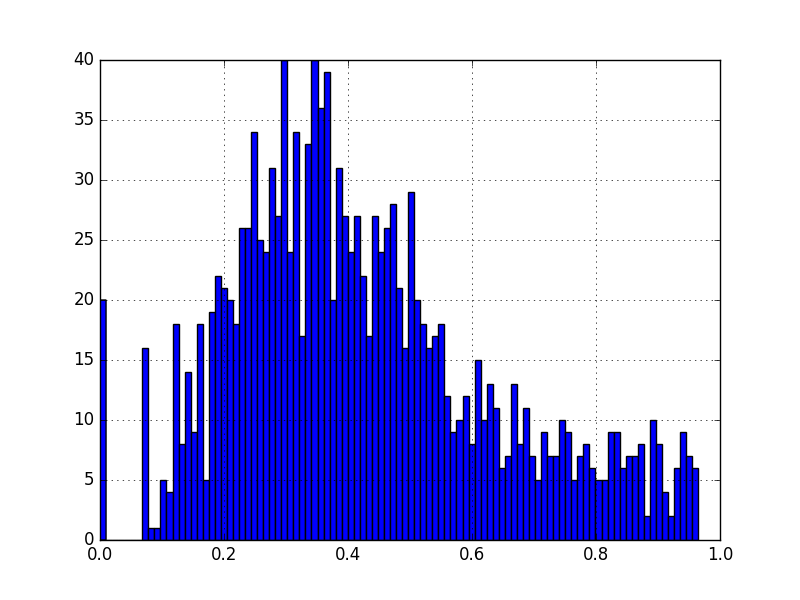
\includegraphics[width=0.75\linewidth]{pics/shapiro_experimental.png}
  \caption{Гистограмма показателя Шапиро-Уилка}
  \label{normality_experimental}
\end{figure}

Из-за существенной ненормальности в данных требуется стандартизация оригинальных данных. Без стандартизации, из-за геометрических идей, лежащих в основе выбранных алгоритмов кластеризации и отбора признаков, наибольшей важностью будут обладать признаки с большой дисперсией, что противоречит постановке задачи из целевой области.